%%
%% This is file `sample-sigconf.tex',
%% generated with the docstrip utility.
%%
%% The original source files were:
%%
%% samples.dtx  (with options: `sigconf')
%% 
%% IMPORTANT NOTICE:
%% 
%% For the copyright see the source file.
%% 
%% Any modified versions of this file must be renamed
%% with new filenames distinct from sample-sigconf.tex.
%% 
%% For distribution of the original source see the terms
%% for copying and modification in the file samples.dtx.
%% 
%% This generated file may be distributed as long as the
%% original source files, as listed above, are part of the
%% same distribution. (The sources need not necessarily be
%% in the same archive or directory.)
%%
%% The first command in your LaTeX source must be the \documentclass command.
\documentclass[sigconf]{acmart}

%%
%% \BibTeX command to typeset BibTeX logo in the docs
\AtBeginDocument{%
  \providecommand\BibTeX{{%
    \normalfont B\kern-0.5em{\scshape i\kern-0.25em b}\kern-0.8em\TeX}}}

%% Rights management information.  This information is sent to you
%% when you complete the rights form.  These commands have SAMPLE
%% values in them; it is your responsibility as an author to replace
%% the commands and values with those provided to you when you
%% complete the rights form.
\setcopyright{acmcopyright}
\copyrightyear{2022}
\acmYear{2022}
\acmDOI{10.1145/1122445.1122456}
%% These commands are for a PROCEEDINGS abstract or paper.
\acmConference[Woodstock '22]{Woodstock '22: ACM Symposium on Neural
  Gaze Detection}{April 4, 2022}{Woodstock, NY}
\acmBooktitle{Woodstock '22: ACM Symposium on Neural Gaze Detection,
  April 4--5, 2022, Woodstock, NY}
\acmPrice{15.00}
\acmISBN{978-1-4503-XXXX-X/18/06}


%%
%% Submission ID.
%% Use this when submitting an article to a sponsored event. You'll
%% receive a unique submission ID from the organizers
%% of the event, and this ID should be used as the parameter to this command.
%%\acmSubmissionID{123-A56-BU3}

%%
%% The majority of ACM publications use numbered citations and
%% references.  The command \citestyle{authoryear} switches to the
%% "author year" style.
%%
%% If you are preparing content for an event
%% sponsored by ACM SIGGRAPH, you must use the "author year" style of
%% citations and references.
%% Uncommenting
%% the next command will enable that style.
%%\citestyle{acmauthoryear}

%%
%% end of the preamble, start of the body of the document source.
\begin{document}

%%
%% The "title" command has an optional parameter,
%% allowing the author to define a "short title" to be used in page headers.
\title{Virtual Reality Sickness: An Investigation of Reduction Methods}

%%
%% The "author" command and its associated commands are used to define
%% the authors and their affiliations.
%% Of note is the shared affiliation of the first two authors, and the
%% "authornote" and "authornotemark" commands
%% used to denote shared contribution to the research.

\author{Christian Bosch}
\email{trekcsb@colostate.edu}
\affiliation{%
  \institution{Colorado State University}
  \city{Fort Collins}
  \state{Colorado}
  \country{USA}
  \postcode{80521}
}

\author{Ryan McCormick}
\email{ryanbmcc@colostate.edu}
\affiliation{%
  \institution{Colorado State University}
  \city{Fort Collins}
  \state{Colorado}
  \country{USA}
}
  
\author{Brendan Nolan}
\email{bpnolan@colostate.edu}
\affiliation{%
  \institution{Colorado State University}
  \city{Fort Collins}
  \state{Colorado}
  \country{USA}
}
\begin{teaserfigure}
  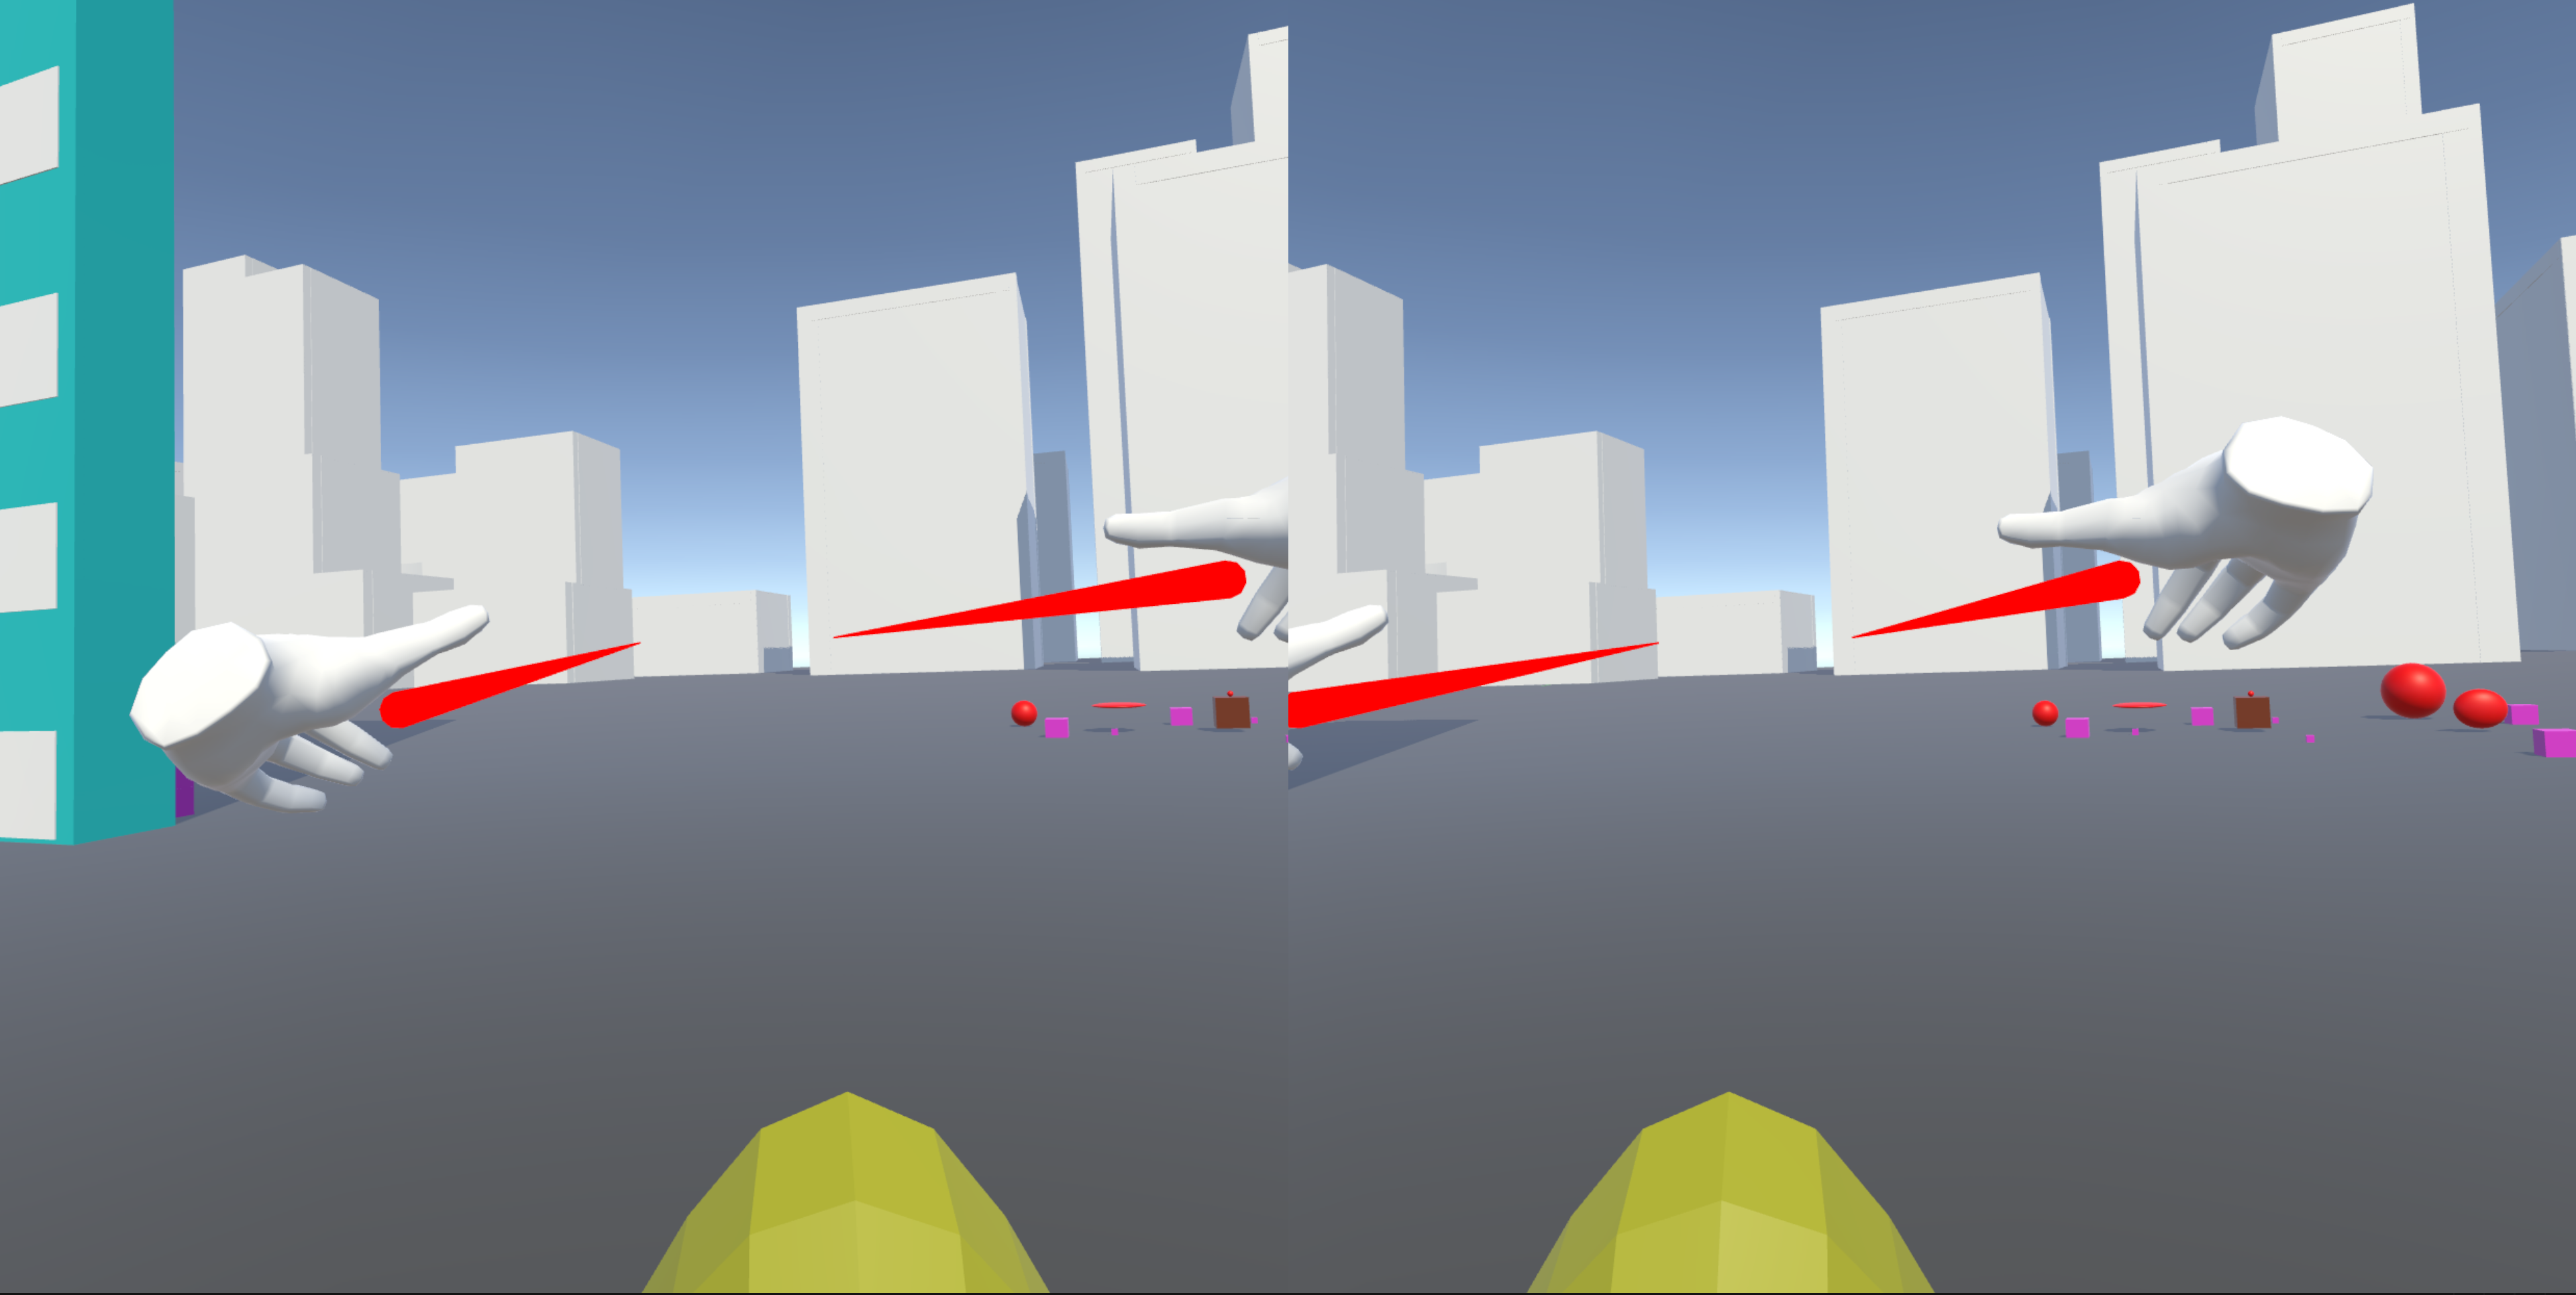
\includegraphics[width=\textwidth]{samples/Nose VR.png}
  \caption{In the virtual environment with an attached nose rest frame.}
  \Description{Nose png}
  \label{fig:teaser}
\end{teaserfigure}
%%
%% By default, the full list of authors will be used in the page
%% headers. Often, this list is too long, and will overlap
%% other information printed in the page headers. This command allows
%% the author to define a more concise list
%% of authors' names for this purpose.
\renewcommand{\shortauthors}{Bosch, et al.}
\begin{abstract}
In this study we attempted to find causes of virtual reality sickness (a type of motion sickness) and how to diminish the symptoms via rest frames. This was done in the hopes to further the field of Virtual Reality by making it more accessible to those who are prone to motion sickness. In experiment 1, we created a virtual environment in which participants utilized a basic locomotion system to test how both controlled (walking, object interaction) and uncontrolled motion (jump-pad jumping/viewing oscillations) affected virtual reality sickness (VRS) symptoms. We found a significant increase in reported symptoms during jump oscillations when compared to both forms of controlled movement. Experiment 2 tested how rest frames affected reported VRS symptoms via no rest frame, static (nose), and dynamic (dot effect) rest frames. We found no significant difference between the conditions; however, rest frames did increase VRS symptoms with dot effect having the highest increase in symptoms.
\end{abstract}
%%
%% The abstract is a short summary of the work to be presented in the
%% article.


%%
%% The code below is generated by the tool at http://dl.acm.org/ccs.cfm.
%% Please copy and paste the code instead of the example below.
%%
\begin{CCSXML}
<ccs2012>
 <concept>
  <concept_id>10010520.10010553.10010562</concept_id>
  <concept_desc>Virtual Reality~Virtual Reality Sickness</concept_desc>
  <concept_significance>500</concept_significance>
 </concept>
\end{CCSXML}

\ccsdesc[500]{Virtual Reality~Virtual Reality Sickness}


%%
%% Keywords. The author(s) should pick words that accurately describe
%% the work being presented. Separate the keywords with commas.
\keywords{datasets, virtual reality (sickness), simulator,  postural instability, sensory conflict, Simulator and Virtual Reality Sickness Questionnaire, field of view}

%% A "teaser" image appears between the author and affiliation
%% information and the body of the document, and typically spans the
%% page.

%%
%% This command processes the author and affiliation and title
%% information and builds the first part of the formatted document.
\maketitle

\section{Introduction}
As virtual reality (VR), not to be confused with augmented reality or mixed reality\cite{rauschnabel22}, continues to expand in consumer markets at a rapid pace (expected market cap of \$12 billion in the next two years \cite{Lee21}), the need for sustainable experiences with reduced instances of motion sickness is a must. Motion sickness (MS) is a common occurrence for one in three people whether it be riding in a vehicle or experiencing swaying motion \cite{motion}. Those who have never reported experiencing MS tend to feel some form of MS-related discomfort when first introduced to virtual reality and can experience more severe symptoms with continued exposure. 

\subsection{Motion Sickness and Virtual Sickness}
While there are now more companies picking up the idea of virtual reality, they struggle to deal with the common user issue of virtual reality sickness (VRS), a type motion sickness due to interacting with virtual reality through a head-mounted display (HMD). Motion sickness is caused by your brain receiving conflicting information from different motion sensing parts of the body such as your eyes, inner ear, and various joints \cite{motion}. When these streams of information conflict with each other enough, the brain loses track of whether you are moving. This sensation then causes the body to feel sick and in some cases lose balance \cite{chang20, kennedy10}. Virtual sickness produces the same effects and is caused in part by the same types of information conflicts in the brain, however due to the HMD there are more contributors to the disconnect.
\subsection{Theories of VRS}
There are three different theories supported as potential causes of VRS- sensory conflict, postural instability, and rest frame theory. Sensory conflict can be described as inconsistencies between visuals and vestibular senses \cite{ng20}. 

The inner ear is host to part of the vestibular system, a sensory system that helps the brain understand the position of a persons limbs \cite{Hu17}. This includes the arms, legs, torso, and head positions at any given point in time. When the brain receives different information from the vestibular system than whats is being reported by the eyes, it causes it to lose track of what is really happening to the body, causing symptoms of sickness \cite{stanney20}. 

Rest frames, stationary objects in the VR field-of-view (FOV), can reduce the conflicts the brain receives from the vestibular system \cite{Luks19, chang13}. \cite{cao18} suggests rest frames when viewed can have a stabilizing effect on visual perception. This is due to a static frame allowing the brain to track where it is relative to the space it is seeing around itself \cite{porcino20}.

Postural instability, described as a degradation of stability by \cite{chang12}, can be seen heavily in VR due to the contrast between your eyes perceiving you moving and your body attempting to replicate the movement without actually moving causing a disconnect in postural control \cite{sun20}. 

\subsection{Problem: Development of VRS Symptoms}
Virtual reality is currently not viable for extended use by a large portion of the population due to VRS affecting even those who are not typically susceptible to motion sickness. By taking a deeper dive into the theories above, we will be able to assess the greater symptoms of VRS. In doing so we hope to add to prior research and expand upon the findings to influence future research into finding ways of mitigating the effects of VRS.

\section{Related Work}
There have been many different studies surrounding virtual reality sickness concerning the causes of it as well as what could help to alleviate the symptoms. The high likelihood of developing VRS symptoms has led researchers to develop various techniques in order to reduce the prevalence of VR-related sickness. \cite{teixeira21, fernandes16,shi21} experimented with gradually increasing/decreasing user field-of-view (FOV). The change in the FOV can help to develop a sense of presence in the user. Presence, as defined by \cite{weech19}, is a users sense of being transported from their physical location to a virtual environment as well as being immersed in the environment. This sense of presence and immersion is theorized to alleviate conflicting information that the brain is receiving from the body. \cite{fernandes16, teixeira21} found that restricting the FOV decreased VRS symptoms whereas increasing the FOV also increased severity of symptoms.

Vignetting, the act of darkening or blurring the periphery of users' vision, can contribute to the severity of experience VRS symptoms. In parallel with FOV, it has been shown that increasing vignetting can lead to increased symptoms that can be different per user \cite{norouzi18}. Blurring objects when a user rotates their head has been found to produce nominally lower reported symptoms, however these are not significant \cite{budhiraja17}. Along with vignetting there are other periphery changes that can be made to reduce VRS symptoms, one of which was used in a study conducted by \cite{buhler18}. In thier study they used multiple effects to try and diminish the symptoms one of which was the circle effect. This took the peripheral vision of the user and froze it in place for five seconds before updating to match the focal point of the camera to match the area and lighting. The results of the study showed that there was no significance in reducing VRS symptoms.

The effect of rest frames on virtual reality sickness has been studied over time since virtual reality was first introduced. The rest frame has been used to attempt to reduce the effects and/or onset of VRS. This is primarily done by placing some static object in the peripheral vision of the user to allow their brain to have something to subconsciously focus on. \cite{wienrich18} attempted to find the effect of a virtual nose as a rest frame on the users experienced levels of VRS. While they found that the presence of a virtual nose helped, we plan to conduct our own experiment to support their claim. Another example of a rest frame can be a virtual cockpit as used by \cite{cao17} to give their participants something to focus on as they traversed a post apocalyptic world.

A study specifically looking at static rest frames was done by \cite{somrak21}. In the study, participants were asked to follow a static path indicated by floating coins as fast as possible. In the view of the user was one of three rest frames, nothing, sunglass frames, and the bill of a hat at the top of the view. They found that the sunglasses significantly lowered the symptoms of VRS in those with VR experience and both rest frames, excluding nothing as a rest frame, lowered the symptoms in those who had no prior VR experience.

There are two main methods of movement used in virtual environments, those being teleportation and locomotion. Teleportation is the act of snapping the user from the current position to a predetermined point instantaneously. Locomotion is full user control between the current position and any desired position. \cite{clifton20} found that users reported more VRS when utilizing locomotion opposed to teleportation.

Having a lack of control of ones self and/or surroundings in virtual environment can also be detrimental to VRS symptoms \cite{nurburger21}. \cite{Lin07} tested this by placing a driver in the seat of a stationary car surrounded by walls displaying a road. The screens would then move forward on the road to simulate the vehicle moving. It was reported by the participants that during the experiment they felt a moderate to high level of VRS.

In terms of displays, it has been discussed that stereoscopic and monoscopic displays can lead to VRS as well. In a study done by \cite{rebenitsch16} it was postulated that stereoscopic displays and monoscopic displays can have a different effect on the eyes of a viewer, each leading to their own issues. One such issue is that stereoscopic HMD's have been found to cause an increase in most forms of motion sickness including VRS versus stereoscopic displays. It was also found that stereoscopic displays in general cause more cybersickness and VRS symptoms that monoscopic displays. Other similar factors include latency, flicker, and their affect on virtual sickness\cite{ramaseri22}. Latency, the lag of time between the action input and the action occurring on screen, can contribute to VRS due to the delay in expected actions causing a disconnect between the predicted result and the true result that your brain experiences\cite{stauffert20, kim20}. Flicker, the rapid change in brightness of a display, also contributes to the same effects caused by latency \cite{laviola00}.

Multi-sensory stimulations were studied by \cite{grassini(1)21} in the form of visual, audio-visual, visual with vibrations, and audio-visual with vibrations while using virtual roller coaster. The hope of their study was to find significance in one of these forms reducing symptoms of simulator sickness. However they only found that females experienced a higher sense of presence with vibrations than males. Roller coasters were also used in an experiment conducted by \cite{davis15} to see how the fidelity of two different roller coasters would effect a users level of cybersickness. They found that more realistic roller coasters caused higher levels of cybersickness.

Outside of virtual reality there have been studies conducted to find if oscillating lines have any effect on motion sickness. \cite{koslucher15} ran an experiment to find the effect of oscillating lines on motion sickness between genders. Their participants were placed into a moving room with the walls painted with oscillating lines. It was found that females felt more of an effect from the oscillating lines compared to their male counterparts. 

\begin{comment}
\section{Methodology}
Each study will be conducted with participants attending Colorado State University that will polled prior to the selection about potential visual impairments or medical conditions that would bar them from participation. Prior experience with VR will also be addressed. In order to collect data for our experiments we will use a Virtual Reality Sickness Questionnaire (VRSQ) as noted in Figure 1. The VRSQ is an altered version of the Simulator Sickness Questionnaire that is used to gauge a persons response to the severity of the symptoms induced by a VR experiment \cite{kim18}. This questionnaire is used to obtain qualitative measures of experienced symptoms including nausea, dizziness, headaches, trouble focusing, etc., because symptoms can vary between participants. We considered making the VRSQ inside of the virtual environment as to not cause any break in experience but decided to have it on paper outside of the HMD to allow for a break between studies \cite{putze20}.
\end{comment}

\section{Usability Study}
\subsection{Methods}

\subsubsection{Participants}
Participants were 5 Colorado State University undergraduate students voluntarily consenting to complete this study. Participants (5 male) were between 19 and 27 (M = 23, SD = 3) years old.

\subsubsection{Design}
This study follows a usability study design in which participants followed the procedure for experiment 1. Participants are polled prior to the selection about potential visual impairments or medical conditions that would bar them from participation. Prior experience with VR will also be addressed. This study tested our experimental setup and we were able to receive feedback from participants. Participants were questioned on how they felt, activities performed, and their favorable and non-favorable experiences. We developed the questionnaire (as noted in Figure 1) based on previous studies \cite{kim18, Hunt18, han11, palmisano17, farmani20}.

\subsubsection{Materials}
In this experiment, we used Oculus Quest 2’s as VR headsets linked to a desktop computer (Ryzen 5600X 3.7GHZ, NVidia RTX 3080, 16GB RAM) for VR display output. We used Unity Engine to generate VR environments for participants to complete the study. We will also had participants take a survey after completing the study.

\subsubsection{Procedure}
Participants began by placing the Oculus Quest 2 HMD on their head and beginning the environment program. Participants were given time to adjust to the environment as well as were provided verbal instructions on activities to complete while in the environment. Participants used the locomotion system to maneuver through the environment for 5 minutes. Participants then completed an object interaction task for 5 minutes in which the hand models were outfitted with ray interactors to pick up objects such as cubes and spheres to organize and move however they like. The third activity was interaction with a jump-pad for 5 minutes in which participant were placed directly in front of a red/white target and launched themselves through the air to land in the center of the target. The final task to complete was using the jump-pad to launch into the air and have blue/white oscillating lines placed in front of them to view during their fall to the ground repeatedly for 5 minutes. A usability questionnaire was provided at the end of study with questions about the functionality/layout of the environment and their experience.

\subsection{Discussion}
Participants were able to provide ample feedback after their experiences with the study. After asking if task explanations were adequate or if they preferred in-VR text boxes with instructions, 2 participants agreed that text instructions would have been helpful; however, all participants agreed verbal instruction was good. When prompted on any additional activities they would have to have seen, 3 participants replied that the study had fun activities and 2 participants expressed a desire for more jump-pads or links between jump-pads to maneuver between. When asked their thoughts on the physical layout of the environment and amount of interact-ables, all participants expressed that more interact-ables such as cubes or spheres would be a good addition and that the layout was good for activities. When questioned on the best and and worst things about the study, all agreed it was a combination of jumping and experiencing VRS from the jumping respectively. Additional thoughts included adding more jump-pad activities like bouncing between pads and having more interact-able object types.

\begin{figure}[h]
  \centering
  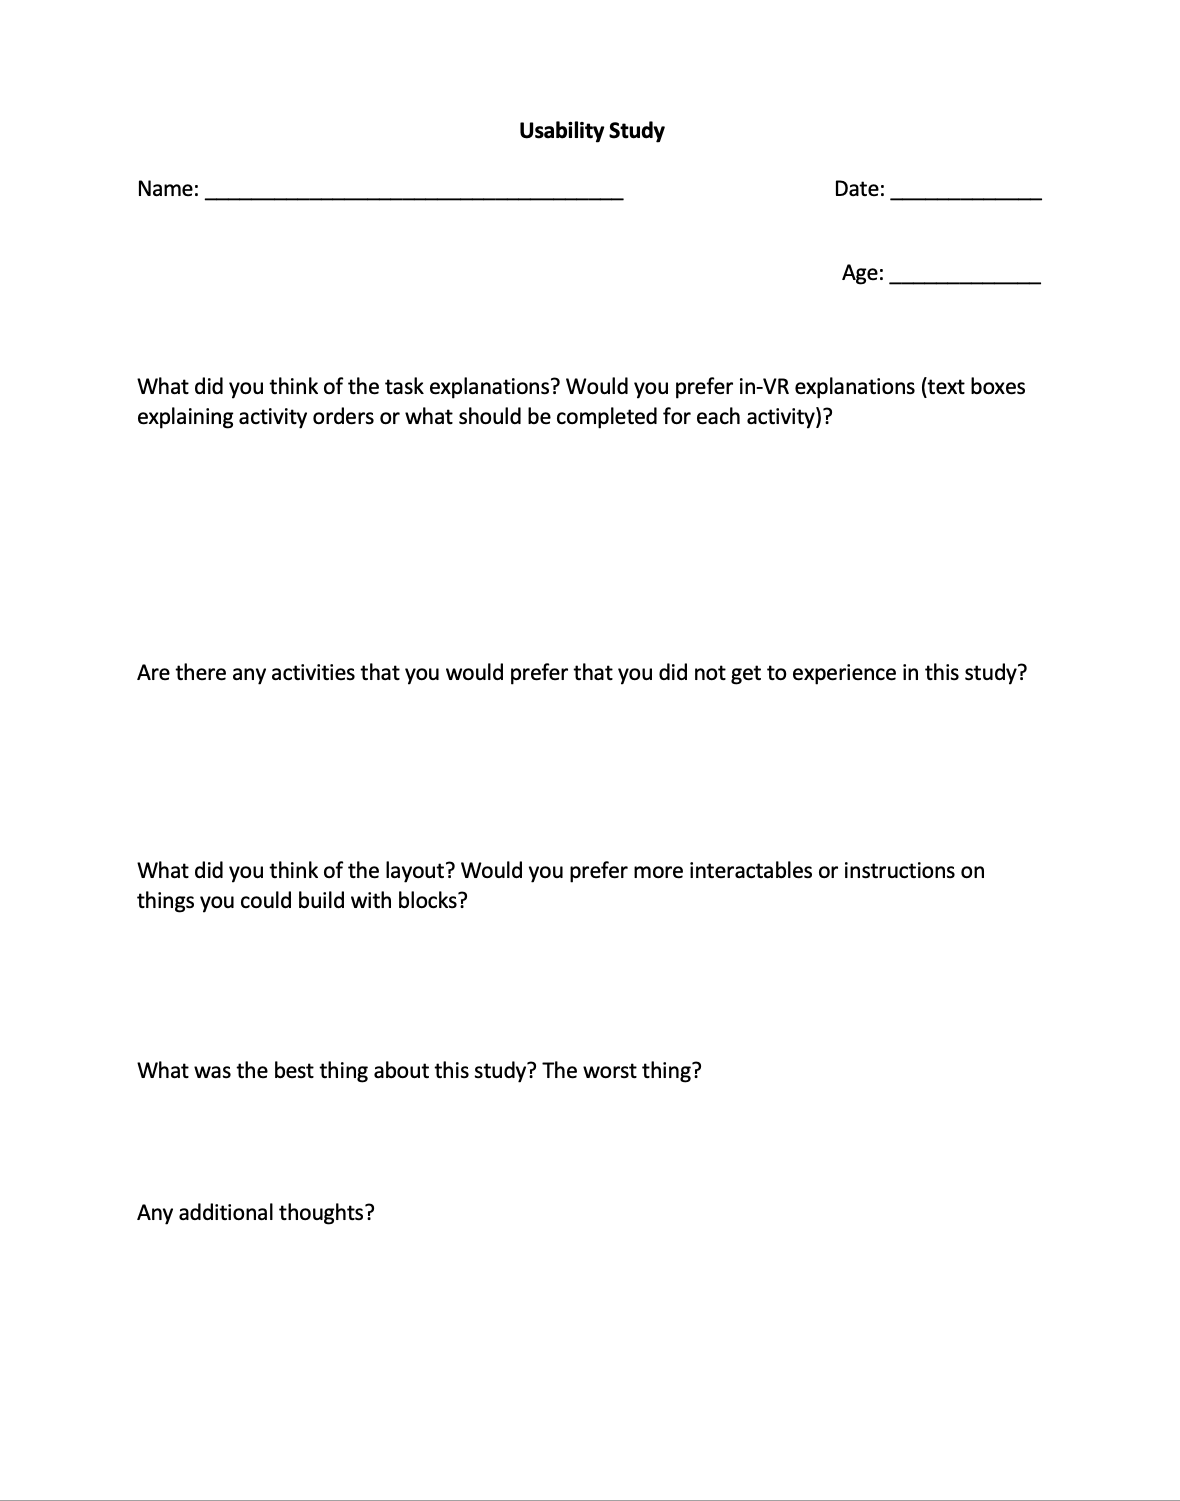
\includegraphics[width=\linewidth]{Usability Q}
  \caption{Usability study questionnaire developed for this study; questions ranged from task explanations, activities, layout, and user experience. Any issues were also noted in the questionnaire such as non/under-performing aspects.}
  \Description{Example of the questionnaire to be used}
\end{figure}



\section{Experiment 1}
\subsection{Methods}

\subsubsection{Participants}
Participants were 7 Colorado residents voluntarily consenting to complete this study. Participants (4 female, 3 male) were between 23 and 59 (M = 38, SD = 15) years old.

\subsubsection{Design}
Our first control study was an extension on a test done by Xavier Hunt and Leigh Ellen Potter \cite{Hunt18}. This study utilized a 1 x 4 (VR activity: walking, object interaction, jump-pad target, jump-pad visual oscillation) design and was manipulated within-subjects. Participants' virtual reality sickness questionnaire (VRSQ) scores were used to evaluate which design choices for VR cause increased motion sickness for users. The purpose of this study was to examine how object interaction and non user-controlled motion affects participants' reported symptoms of VRS. Primary tasks to be completed by participants included traversing/interacting with objects within the VE and subjecting them to non-user controlled movement such as placing them on "jump pads," which pushed their avatar through the air. We hypothesize that uncontrolled movement will have a larger effect on causing symptoms of VRS than controlled movement and object interaction.

\subsubsection{Materials}
In this experiment, we used Oculus Quest 2’s as VR headsets linked to a desktop computer (Ryzen 5600X 3.7GHZ, NVidia RTX 3080, 16GB RAM) for VR display output. We used Unity Engine to generate VR environments for participants to complete the study. We will also had participants take VRSQs after completing each activity.

\subsubsection{Virtual Reality Sickness Questionnaire}
We created a version of the VRSQ, as shown in Figure 2, which checked for 9 different common symptoms of VRS, as noted by \cite{keshavarz11, jang22} including headache, dizziness, fatigue, nausea, etc. Neutral language and only symptoms/severity were included in the VRSQ based on \cite{keshavarz11} suggesting utilizing neutral language in VRSQs as to not elicit increased perceptions of motion sickness. \cite{sevinc20} created a version of the sickness questionnaire utilizing multiple systems of questionnaires including simulator sickness qustionnaire (SSQ), cybersickness questionnaire (CST), F-SSQ, and VRSQ; however, we adopted use of the VRSQ for related results in VR. The VRSQ is scored from 0-27 based on the severity of each symptom (none = 0, slight = 1, moderate = 2, severe = 3). The total of scores is calculated and expressed as an overall VRS symptom score. 

\begin{figure}[h]
  \centering
  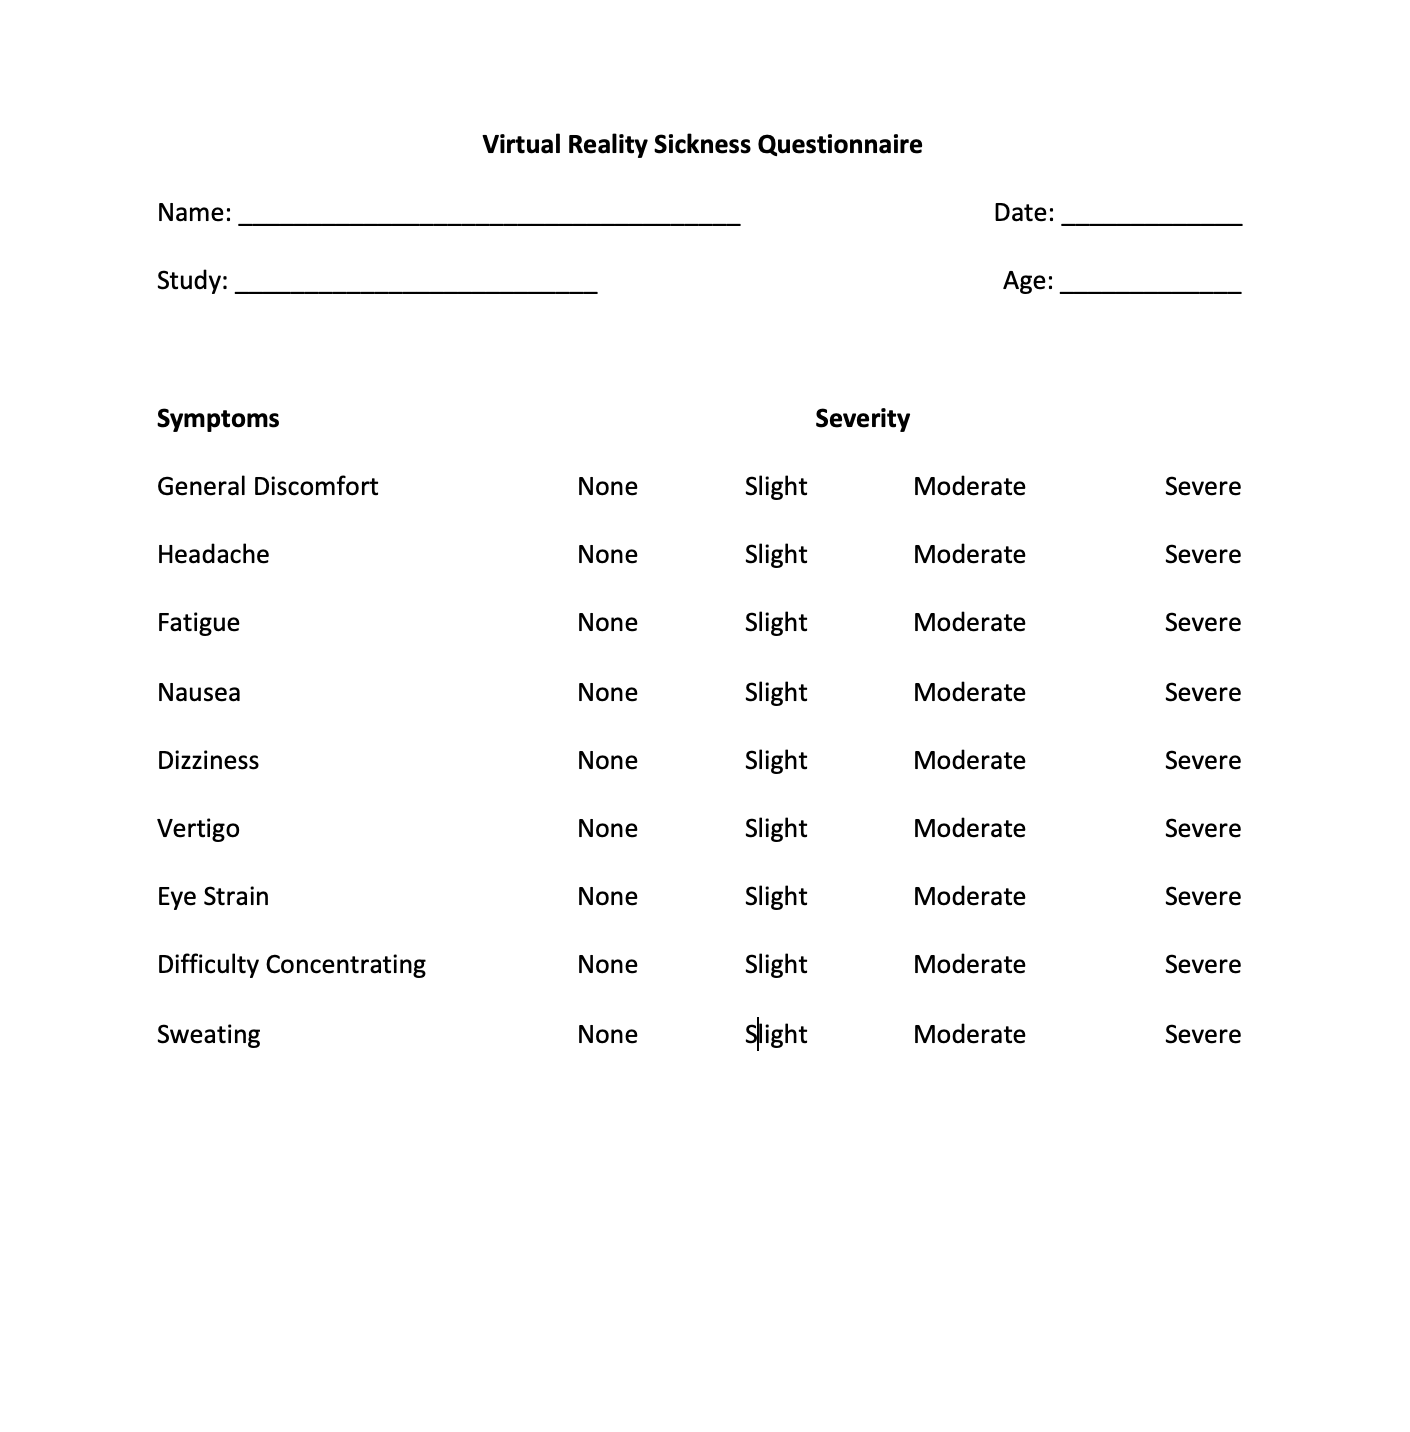
\includegraphics[width=\linewidth]{samples/VRSQ.png}
  \caption{Virtual reality sickness questionnaire developed for this study; includes symptom/severity relationships rated on scores from 0-27 (0 being asymptomatic and 27 being extremely severe).}
  \Description{Example of the questionnaire to be used}
\end{figure}

\subsubsection{Procedure}
Participants began by placing the Oculus Quest 2 HMD on their head and beginning the environment program. Participants were given time to adjust to the environment as well as were provided verbal instructions on how to move and interact with objects as well as activities to complete while in the environment. Participants used the locomotion system to maneuver through the environment for 5 minutes. Participants then completed an object interaction task for 5 minutes in which the hand models were outfitted with ray interactors to pick up objects such as cubes and spheres to organize and move however they like. The third activity was interaction with a jump-pad for 5 minutes in which participant were placed directly in front of a red/white target and launched themselves through the air to land in the center of the target. The final task to complete was using the jump-pad to launch into the air and have blue/white oscillating lines placed in front of them to view during their fall to the ground for 5 minutes. VRSQs were completed after every activity to measure sickness symptoms. 

\subsection{Results}
A 1 x 4 (VR activity: walking, object interaction, jump-pad target, jump-pad visual oscillation) repeated measures ANOVA was conducted to analyze differences in users' reported VRSQ scores between activities. Overall, a significant effect was found for the study (\textit{F}(3, 18) = 9.04, \textit{p} < .001). Follow-up t-tests showed reported VRSQ scores for jump oscillations were significantly higher (\textit{M} = 7.29, \textit{SD} = 5.50) than walking (\textit{M} = 2.86, \textit{SD} = 2.73), \textit{t}(6) = 3.92, \textit{p} = .008, \textit{d} = 1.48. VRSQ scores for jump oscillations were also significantly higher than object interaction (\textit{M} = 2.86, \textit{SD} = 3.93), \textit{t}(6) = 4.94, \textit{p} = .003, \textit{d} = 1.87. VRSQ scores between both walking (\textit{M} = 2.86, \textit{SD} = 2.73) and object interaction (\textit{M} = 2.86, \textit{SD} = 3.93) were shown to be identical. VRSQ scores for jump oscillation were higher than jump target (\textit{M} = 4.57, \textit{SD} = 4.86); however, the difference was close-to but not significant, \textit{t}(6) = 2.41, \textit{p} = .05, \textit{d} = 0.91. All other comparisons were shown to be non-significant. 

\begin{figure}[h]
  \centering
  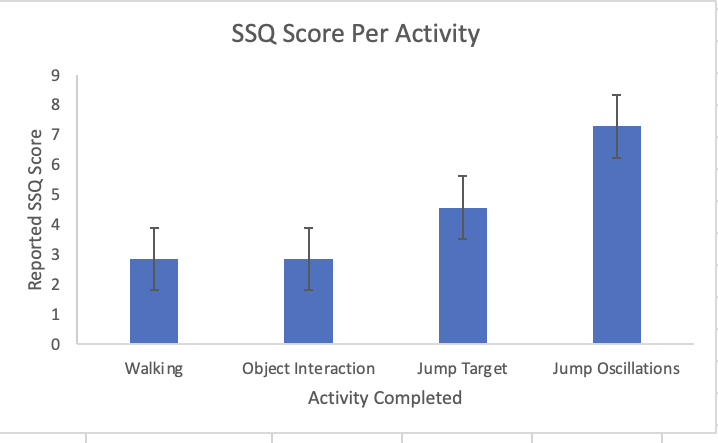
\includegraphics[width=\linewidth]{samples/C1 Graph.png}
  \caption{Averaged VRSQ scores across each activity. Walking and object interaction had the same score (2.86) whereas jump target had a score of 4.57 and jump oscillations had a score of 7.29. A significant difference was measured between both walking/object interaction and jump oscillations.}
  \Description{Graph of Control 1 Data}
\end{figure}

\begin{table}
  \caption{Experiment 1 Descriptives}
  \label{tab:commands}
  \begin{tabular}{ccl}
    \toprule
    Activity & \textit{M} & \textit{SD}\\
    \midrule
    \texttt{Walking} & 2.86 & 2.73 \\
    \texttt{Object Interaction}& 2.86 & 3.93\\
    \texttt{Jump Target}& 4.57& 4.86\\
    \texttt{Jump Oscillations}& 7.29 & 5.50\\
    \bottomrule
  \end{tabular}
\end{table}

\subsection{Discussion}
Recorded VRSQ scores were shown to be within our original predictions between motion and uncontrolled motion; however, most comparisons were shown to be non-significant or having identical scores. Unexpectedly, walking and object interaction scores were the same and higher object interaction scores were expected. This shows there is no discernible difference in perceived VRS symptoms between walking and viewing our environment through an HMD and interacting with objects within the environment. Walking/object-interaction  and jump oscillations was a significant difference, showing that uncontrolled motion (jumping and falling) while viewing similarly defined meshes and textures has a significant effect on perceived VRS symptoms. 


\section{Experiment 2}
\begin{figure*}[h]
  \centering
  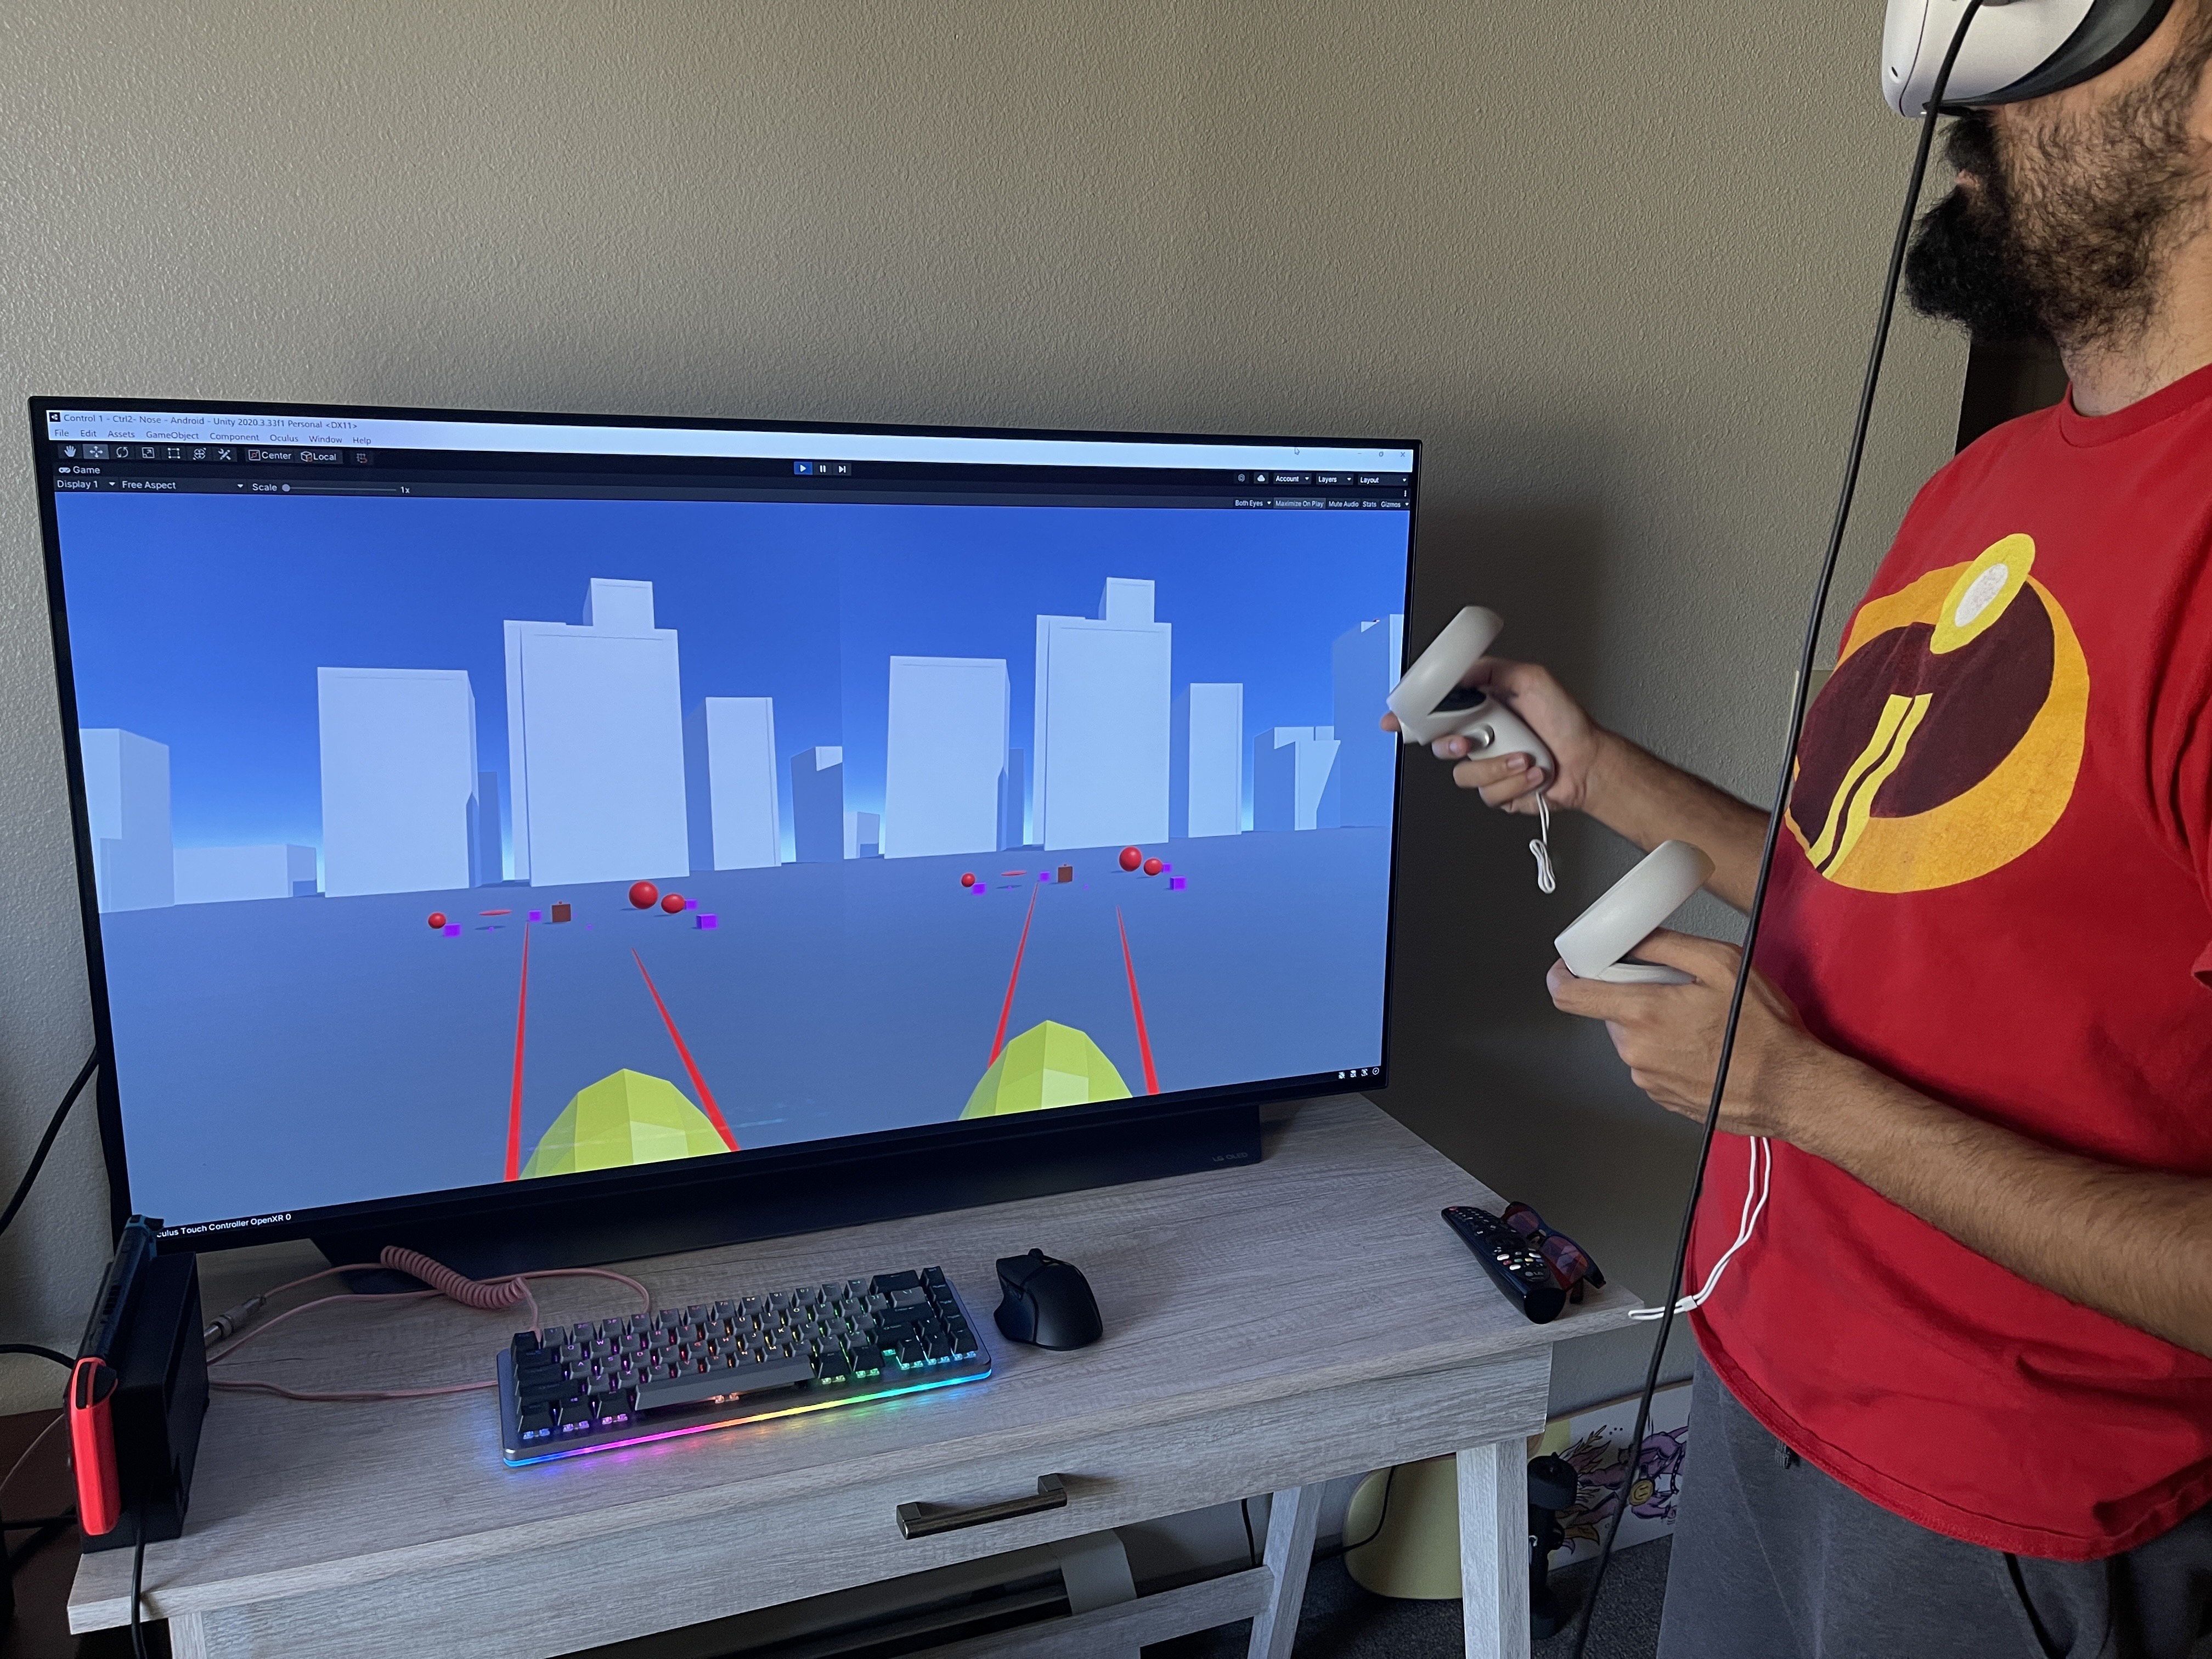
\includegraphics[width=\linewidth]{samples/IMG_1811.jpg}
  \caption{Project contributor Ryan McCormick demonstrating the nose rest frame scene in Unity using the Oculus Quest 2. The scene is displayed through both eyes so the image is displayed twice (one for left eye and one for right).}
  \Description{Ryan nose RF scene}
\end{figure*}
\subsection{Methods}

\subsubsection{Participants}
The participants for experiment 2 were six Colorado resident volunteers that consented to participate in the study. Participants (1 female, 5 males) were between 20 and 22 (M = 21, SD = 1) years old.

\subsubsection{Design}
Our second control study was built off of our previous control with the addition of two different rest frames from the GingerVR package on GitHub \cite{ang}. The purpose of this study was to measure reported differences such as dizziness, trouble focusing, and nausea \cite{jung17, saredakis20, bockelman17}, if any, between static and dynamic rest frames using a VRSQ \cite{buhler18}. This study utilized a 1 x 3 (Rest frame type: None, Nose, Dot Effect) design and was manipulated within-subjects. The experiment was also counter balanced to account for ordering effects. The first rest frame that was implemented was a static nose that sits just below the center of view in the middle of the participants eyes. The second rest frame was a grid of dots that would dynamically move at twice the speed of the user relative to the direction they were facing. Both of these rest frames were tested using the same tasks. These being controlled movement via user controlled locomotion, uncontrolled movement via jump pads launching the user into the air on contact, and object interaction. The environment was a flat plain with buildings surrounding the perimeter, jump pads to get on top of the buildings, and interact-able cubes and spheres. We hypothesize that the rest frames will have a diminishing effect on VRS symptoms over a non-rest frame experience.

\subsubsection{Materials}
In this experiment, we used Oculus Quest 2’s as VR headsets linked to a desktop computer (Ryzen 5600X 3.7GHZ, NVidia RTX 3080, 16GB RAM) for VR display output. We used Unity Engine to generate VR environments for participants to complete the study. We will also had participants take a survey after completing the study.

\subsubsection{Procedure}
Participants began by placing the Oculus Quest 2 HMD on their head and starting the environment program. Participants were given time to adjust to the environment as well as provided verbal instructions on how to move and interact with objects. The participants were instructed to spend 5 minutes interacting with the blocks and spheres that surrounded them, building or throwing them around, and spend 5 minutes exploring the environment using the jump pads to get on top of the buildings around them. After the ten minute period, the user would then remove the HMD, fill out the VRSQ, and take a five minute break. During this time the experiment was reset and changed to the next type of rest frame. This was completed a total of three times per participant as to complete each of the three types of rest frames in the experiment. 

\subsection{Results}
A 1 x 3 (Rest frame type: None, Nose, Dot Effect) repeated measures ANOVA was conducted to analyze differences in reported VRSQ scores between different variations of static and dynamic rest frames in VR. The ANOVA showed no overall significant effect of rest frames on perceived VRSQ symptoms between all tested activities in VR (walking, object interaction, and jump-pad building maneuvering), (\textit{F}(2, 10) = 2.83, \textit{p} < .11). Follow up t-tests showed that nose VRSQ scores were higher (\textit{M} = 4.83, \textit{SD} = 4.36) than using no rest frame (\textit{M} = 4.17, \textit{SD} = 3.19); however, the difference was non-significant, \textit{t}(5) = 0.51, \textit{p} = .63, \textit{d} = 0.21. The dot effect rest frame also had higher reported VRSQ scores (\textit{M} = 6.83, \textit{SD} = 5.19) than using no rest frame, but the difference was non-significant, \textit{t}(5) = 1.84, \textit{p} = .13, \textit{d} = 0.75. The dot effect rest frame had a significantly higher reported VRSQ score than using a nose rest frame, \textit{t}(5) = 3.87, \textit{p} = .01, \textit{d} = 1.58. 

\begin{figure}[h]
  \centering
  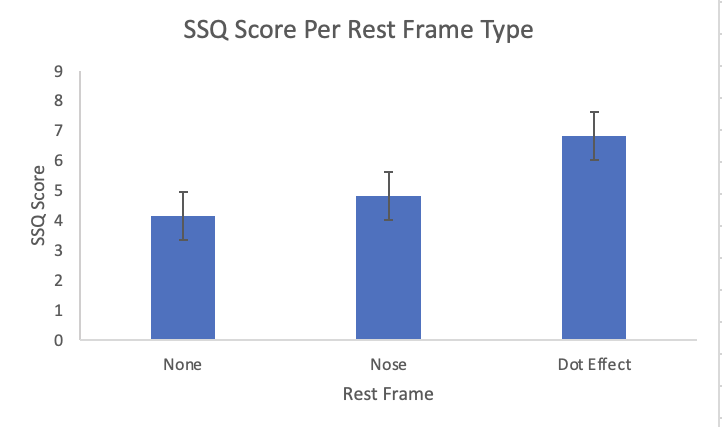
\includegraphics[width=\linewidth]{samples/C2 Graph.png}
  \caption{Averaged VRSQ scores across each type of rest frame condition. No rest frame had an VRSQ score of 4.17, the nose rest frame had a score of 4.83, and the dot effect had a VRSQ score of 6.83. Both rest frame and dot effect were higher than the control using no rest frame.}
  \Description{Graph of Control 2 Data}
\end{figure}

\begin{table}
  \caption{Experiment 2 Descriptives}
  \label{tab:commands}
  \begin{tabular}{ccl}
    \toprule
    Rest Frame & \textit{M} & \textit{SD}\\
    \midrule
    \texttt{None} & 4.17 & 3.19 \\
    \texttt{Nose}& 4.83 & 4.36\\
    \texttt{Dot Effect} & 6.83 & 5.19\\
    \bottomrule
  \end{tabular}
\end{table}

\subsection{Discussion}
Our results for experiment 2 were unexpected as we did not anticipate rest frames having the opposite intended effect on VRS symptoms. The rest frames were intended to reduce VRS symptoms by acting a stable figure in the HMD while participants were immersed in the virtual environment; however, they increased average scores over the control in the case of the nose, and significantly higher in the case of the dot effect. This could be due to the placement of the nose in the users' field-of-view (FOV) or the dot effect using too large of dots/matrix size. A small sample size could have had an effect on the distribution of participant scores causing rest frame scores to be higher. One participant reported a score of 15 after completing the dot effect scenario which was roughly double the standard deviation of that condition, so that outlier could have contributed to a greater average score for the dot effect. More investigation into why these rest frames had an increasing effect on VRS symptoms will need to be completed whether it stem from the virtual environment or the adaptation of the rest frames within the study having unintended effects.

\section{Conclusion}
In our study, we attempted to find design aspects that increased perceived symptoms of VRS and methods of utilizing static and dynamic rest frames to attempt to lower symptoms. Experiment 1 tested how locomotion (walking), object interaction, and uncontrolled movement variations (jump target, jump oscillations) affected participants and how any symptoms of VRS would increase or decrease. Inline with our hypothesis, we found jump oscillations had a significant increase of symptoms over basic locomotion and object interactions via ray interactors. Experiment 2 aimed to test if rest frames were effective at diminishing VRS symptoms via static (nose) and dynamic (dot effect) rest frame variations. Unexpectedly, both variations of rest frames caused an increase in VRS symptoms over a non-rest framed experience with the dot effect having the highest VRSQ scores. This could be due to small sample size; however, more research will need to be conducted into how rest frames affect user experience in VR. 

%%
%% The next two lines define the bibliography style to be used, and
%% the bibliography file.
\bibliographystyle{ACM-Reference-Format}
\bibliography{References}

%%
%% If your work has an appendix, this is the place to put it.
\appendix



\end{document}
\endinput
%%
%% End of file `sample-sigconf.tex'.
